\section{Evaluation}
\label{s_Evaluation}
% Decide whether this should be a chapter for the entire evaluation including setup and description of datasets baselines etc. or if this should focus on results and discussion only (then rename and move the rest to the methodology chapter)

This chapter assesses the performance and effectiveness of \gls{cftgnn}.

\subsection{Experimental Setup}
\label{s_Evaluation_Setup}

\subsubsection{Factual Baselines}
\label{s_Evaluation_Setup_FactualBaselines}

\subsubsection{Datasets}
\label{s_Evaluation_Setup_Datasets}

\subsubsection{Metrics} % Should this be a chapter here, part of the results section, or part of methodology? 
\label{s_Evaluation_Setup_Metrics}
The choice of appropriate metrics is crucial for evaluating the effectiveness of explanation methods, as it allows for a fair and comprehensive assessment of their performance. As discussed in Sectio \ref{s_ProblemFormulation_Objectives}, the primary objectives of the explainer are maximizing discoveries and minimizing complexity. To judge how well \gls{cftgnn} achieves these objectives, appropriate metrics are required.

The fidelity metric has been proposed to evaluate the quality of explanations \cite{amara_graphframex_2022}. Prior research has established different definitions for the fidelity metric \cite{yuan_explainability_2020, lucic_cf-gnnexplainer_2022, xia_explaining_2023, amara_graphframex_2022}. This work adapts the scores $fid_+$ and $fid_-$ \cite{amara_graphframex_2022, yuan_explainability_2020} to explanations on dynamic graph models.

\begin{equation}
    fid_+ = 1 - \frac{1}{N} \sum_{i = 1}^N \mathbbm{1}(p(f(\mathcal{G}(t_i)), \varepsilon_i) = p(f(\mathcal{G}(t_i) \setminus \mathcal{X}_{\varepsilon_i}, \varepsilon_i))) 
\end{equation}

\begin{equation}
    fid_- = 1 - \frac{1}{N} \sum_{i = 1}^N \mathbbm{1}(p(f(\mathcal{G}(t_i)), \varepsilon_i) = p(f(\mathcal{X}_{\varepsilon_i}, \varepsilon_i)))
\end{equation}

Here, $\varepsilon_1, ..., \varepsilon_N$ are possible future links and $\mathcal{X}_{\varepsilon_1},...,\mathcal{X}_{\varepsilon_N}$ the associated explanations for their prediction. The indicator function $\mathbbm{1}(a = b)$ returns $1$, if $a$ is equal to $b$, else it return $0$.

The $fid_-$ score measures how well the explanation captures the relevant past events that lead the dynamic graph model to its prediction. Thus, it measures the sufficiency of the explanations and is most useful for judging the quality of factual explanations \cite{amara_graphframex_2022}. More relevant to counterfactual explanations is the $fid_+$ score, which measures whether the prediction changes when the explanation is removed from the set of past events. Hence, it provides insights into the necessity of the explanations \cite{amara_graphframex_2022}. Recalling the definition of a counterfactual example from Section \ref{s_ProblemFormulation_CFExamples}, the $fid_-$ score represents the proportion of cases in which the explainer manages to find a counterfactual example, directly accounting for the objective of maximizing discoveries.

% Characterization score?

Addressing the second objective of minimizing complexity, the sparsity metric is a widely used tool to gauge the complexity of explanations \cite{yuan_explainability_2020, amara_graphframex_2022, prado-romero_survey_2023}. It measures the ratio between the past events in the explanation $\mathcal{X}_{\varepsilon_i}$ and all past events considered as candidates for the explanation $C(\mathcal{G}, \varepsilon_i, k, m_{max})$.

\begin{equation}
    sparsity = \frac{1}{N} \sum_{i = 1}^N \frac{|\mathcal{X}_{\varepsilon_i}|}{|C(\mathcal{G}, \varepsilon_i, k, m_{max})|}
\end{equation}

% Fidelity

% Sparsity

% Oracle calls?

% Stability??

% Runtime/Duration

% 


\subsubsection{Infrastructure}
\label{s_Evaluation_Setup_Infrastructure}
Experiments were conducted on a high-performance computing cluster with specific hardware configurations tailored to the datasets used. For the UCI dataset, each experiment was allocated eight cores of an Intel Xeon Gold 6230 CPU with 40 cores, 16GB of RAM storage, and an NVIDIA Tesla V100 SXM2 GPU with 32GB of VRAM. Similarly, for the Wikipedia dataset, each experiment utilized eight cores of an Intel Xeon Platinum 8358 CPU with 64 cores, 16GB of RAM storage, and an NVIDIA Tesla A100 GPU with 80GB of VRAM.

This setup ensures efficient resource utilization and experiments with replicable results.

\subsection{Results}
\label{s_Evaluation_Results}

\subsubsection{Explanation Performance}
\label{s_Evaluation_Results_Performance}


\begin{table}
    \centering
    \begin{tabular}{cccccccccc}
    \hline
         &  \multicolumn{4}{c}{UCI}&  \multicolumn{4}{c}{Wikipedia}& \\
         &  $fid_+$&  $fid_-$&  $sparsity$&  $sparsity_{all}$&  $fid_+$&  $fid_-$&  $sparsity$&  $sparsity_{all}$& \\
         \hline
         PGExplainer&  &  &  &  &  &  &  &  & \\
         TGNNExplainer&  &  &  &  &  &  &  &  & \\
         Greedy Random&  $0.280$&  $0.050$&  $0.039$& $ 0.024$&  &  &  &  & \\
         Greedy Closest&  $0.010$&  $0.010$&  $0.023$&  $0.022$&  &  &  &  & \\
         Greedy Recent&  $0.610$&  $\textbf{0.425}$&  $0.044$&  $0.048$&  &  &  &  & \\
 Greedy 1-best& $0.640$& $0.285$& $0.029$& $0.044$& & & & &\\
 CoDy Random& $0.655$& $0.315$& $0.044$& $0.086$& & & & &\\
 CoDy Closest& $0.630$& $0.215$& $0.080$& $0.078$& & & & &\\
 CoDy Recent& \underline{$0.660$}& $0.385$& $0.070$& $0.097$& & & & &\\
 CoDy 1-best& $\textbf{0.675}$& \underline{$0.400$}& $0.066$& $0.087$& & & & &\\
 \hline
    \end{tabular}
    \caption{Caption}
    \label{tab:my_label}
\end{table}


\begin{figure}
    \centering
    % This file was created with tikzplotlib v0.10.1.
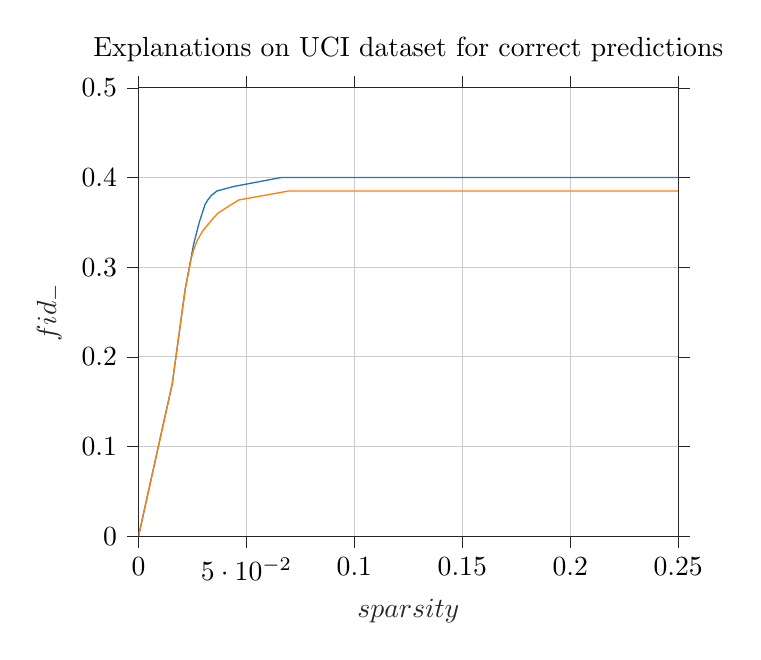
\begin{tikzpicture}

\definecolor{darkorange25512714}{RGB}{255,127,14}
\definecolor{darkslategray38}{RGB}{38,38,38}
\definecolor{lightgray204}{RGB}{204,204,204}
\definecolor{steelblue31119180}{RGB}{31,119,180}

\begin{axis}[
axis line style={darkslategray38},
tick align=outside,
title={Explanations on UCI dataset for correct predictions},
x grid style={lightgray204},
xlabel=\textcolor{darkslategray38}{$sparsity$},
xmajorgrids,
xmajorticks=true,
xmin=0, xmax=0.25,
xtick style={color=darkslategray38},
y grid style={lightgray204},
ylabel=\textcolor{darkslategray38}{$fid_-$},
ymajorgrids,
ymajorticks=true,
ymin=0, ymax=0.5,
ytick style={color=darkslategray38}
]
\addplot [line width=0.48pt, steelblue31119180]
table {%
0 0
0.015625 0.17
0.0215909090909091 0.275
0.0254807692307692 0.325
0.028125 0.35
0.0308277027027027 0.37
0.0320833333333333 0.375
0.0337171052631579 0.38
0.036323051948052 0.385
0.0440705128205128 0.39
0.066015625 0.4
1 0.4
};
\addplot [line width=0.48pt, darkorange25512714]
table {%
0 0
0.015625 0.17
0.0215909090909091 0.275
0.024445564516129 0.31
0.025634765625 0.32
0.0272253787878788 0.33
0.0296415441176471 0.34
0.03125 0.345
0.0347711267605634 0.355
0.0366753472222222 0.36
0.0398116438356164 0.365
0.0430743243243243 0.37
0.0464583333333333 0.375
0.0579769736842105 0.38
0.0696022727272727 0.385
1 0.385
};
\end{axis}

\end{tikzpicture}

    \caption{Caption}
    \label{fig:enter-label}
\end{figure}


\subsubsection{Influence of Selection Criterion}
\label{s_Evaluation_Results_CriterionInfluence}

\subsubsection{Runtime}
\label{s_Evaluation_Results_Runtime}

\subsubsection{Interesting Findings} % Should have a proper name, maybe also multiple subchapters depending on what I can find




% GraphFramEx calls for evaluating correct and wrong predictions separately
